%File: formatting-instruction.tex
\documentclass[letterpaper]{article}
\usepackage{url,graphicx,xcolor}
\usepackage{times}
\usepackage{helvet}
\usepackage{courier}
%\usepackage[guidelines]{faikrmod3}
\usepackage[]{faikrmod3} % without guidelines
\frenchspacing
\setlength{\pdfpagewidth}{8.5in}
\setlength{\pdfpageheight}{11in}

\usepackage{hyperref}

% THE \pdfinfo /Title AND /Author ARE NOT NECESSARY, THEY ARE METADATA FOR THE FINAL PDF FILE
\pdfinfo{
/Title (Bayesian network with Pokemon)
/Author (Alberto Genovese, Christian Di Buò)}
\setcounter{secnumdepth}{0}  
 \begin{document}
% The file aaai.sty is the style file for AAAI Press 
% proceedings, working notes, and technical reports.
%
\title{Bayesian network with Pokemon}
\author{Alberto Genovese, Christian Di Buò\\
Master's Degree in Artificial Intelligence, University of Bologna\\
\{ alberto.genovese5, christian.dibuo \}@studio.unibo.it
}
\maketitle


\attention{DO NOT MODIFY THIS TEMPLATE - EXCEPT, OF COURSE FOR TITLE AND AUTHORS. REMOVE THE \texttt{guidelines} OPTION FROM  \texttt{$\backslash$usepackage[guidelines]\{faikrmod3\}} IN THE \LaTeX\ SOURCE IN THE FINAL VERSION.}

\begin{abstract}
\begin{quote}
This mini-project aims to build and test a Bayesian Network based on the battles of the Pokémon video game. We created two different Bayesian Networks to compare their behaviour and we test them against online players using the showdown battle simulator. We found that the bigger network had a worse performance with respect to the smallest one, and both of them can't do equal or better than the classical search algorithm Iterative Deepening.


\explanation{
This mini-project aims to ... \\
We use ... \\
We found that ...
}

\end{quote}
\end{abstract}


\section{Introduction}
\subsection{Domain}
The Pokémon game is based on battles between two players, in which the objective is to defeat all the opponent player's Pokémon. Every player has a team of six Pokémon, each one with four moves that can either inflict damage or modify the statistics of a Pokèmon. During every turn the player can either decide to use one of the four moves or switch the Pokémon with another one in the team. The move can be enhanced or weaken by the type, or the stats, of the Pokémon.
Our work take inspiration from the "showdown" project \cite{bot}, from which we have made a fork, in this way we have had the opportunity to use their structure for the bot playing on the online pokemon battle simulator \cite{showdown}.

\explanation{
Introduce your work: what you are modelling, if you are drawing inspiration from an existing model, study, paper, textbook example, challenge, \dots.\\
%
Briefly provide whatever background information on the domain you think is necessary for the reader to understand the model and your design choices.
}

\attention{HERE AND EVERYWHERE ELSE: ALWAYS KEEP IN MIND THAT, CRUCIALLY, WHATEVER TEXT/CODE/FIGURES/IDEAS/... YOU TAKE FROM ELSEWHERE MUST BE CLEARLY IDENTIFIED AND PROPERLY REFERENCED IN THE REPORT.}

\subsection{Aim}
The Objective of this project is to understand the capabilities of the Bayesian Network in predicting the best action in a complex environment, in this case, in a game with few choice, but with a great number of variables. This capabilities will be principally compared to other AI method and we will try different composition of the Bayesian Network, by varying the number of nodes and number of discrete value.

\explanation{
Explain the purpose of your project: what do you intend to observe/try/experience/\dots? \\
\begin{itemize}
    \item 
Example: the purpose of this project is to implement part of the Bayesian network described in \cite{10.1371/journal.pone.0220065} and experiment with concepts seen in class \\
%
\item Another example: our aim was to experiment the effect of discretization of continuous variables \\
%
\item Yet another example: we are interested in comparing the run-time and error of approximate inference under different conditions
%
\item One final example: we studied \textit{value of information}: something mentioned in class but not covered in this module, which sparked our interest.
\end{itemize}
}

\subsection{Method}
The Dataset, used along the project, has been created taking around 100 replays of past battles, available as html file in the website showdown \cite{showdown}. It has been written a parser file able to extract the features and automatically create a Dataset as csv file.
The Dataset has been subject of the followings preprocessing activity:
\begin{itemize}
    \item continuous features which have been discretized using the KbinsDiscretizer of the sci-kit learn library. (The ranges have been chosen trying to have a good distribution of values)
    \item aggregation of variables into new variables, such as Enemy Type and Move Type into multiplicator, to indicate the advantage of a move or Pokèmon.
\end{itemize}
To predict the two target variables "choose", for the choice of the move, and "switch" we have built two different Bayesian Networks, using the library pgmpy, the two target can have as value 0 and 1, selected and not selected.
We have built two version of the networks one with an higher number of variables and values, one with a lower number to compare their behaviour and performances.
In the second version of the Bayesian networks, it has been decided to remove the less important nodes, remaining only the ones that, based on the knowledge of the domain, were the most important. This has been done for both of the networks.

\explanation{
Describe the methodology you followed
\begin{itemize}
    \item 
Example: we used pgmpy library methods\footnote{This is just an example: indeed, it is NOT necessary to use pgmpy; the coding language doesn't have to be python either. Feel free to use whatever software framework suits your needs.} to implement our network and run queries. To understand if differences in models, queries, parameters or number of samples induced differences in accuracy, we varied evidence nodes, conditional probability distributions, inference method, ...
\end{itemize}
}

\subsection{Results}
Our exploration reveals that the network, with a big number of variables, gives often a 50\% of probability for the choice of the move or the switch, resulting in an inaccurate selection. While the network with the smaller number of variables rarely gives the same problem.

\explanation{
In a few lines: what are the most noteworthy results you have observed or things you have learned/understood from this project? (only the highlights: there will be a dedicated paragraph for presenting results in the Analysis section)
}

\section{Model}
In the BNs built for this study each node represents a unique random variable. These random variables include among the others "Stab", a boolean random variable, which represent the boost given to the move from the types of the Pokémon, "Boost", which is the enhancement, or the weakening, to the stats of Pokémon and "Multiplicator" that represents the relationship between the type of the target move and the types of the opponent's Pokémon.
To estimate the Conditional Probability Distributions (CPDs) we have used the Bayesian Estimator.
The connections between the variables have been deduced by analyzing the domain: all the variables are pair-wise independent, except for "Choose" and "Switch", which completely depends from all the other variables.
However the model does not take into account all the possible variables, since we do not have access to all the data of the battles.
\explanation{
Insert a picture of your Bayesian network(s) (Figure~\ref{fig:network})
}
\begin{figure}[!ht]
  \centering
  \subfloat{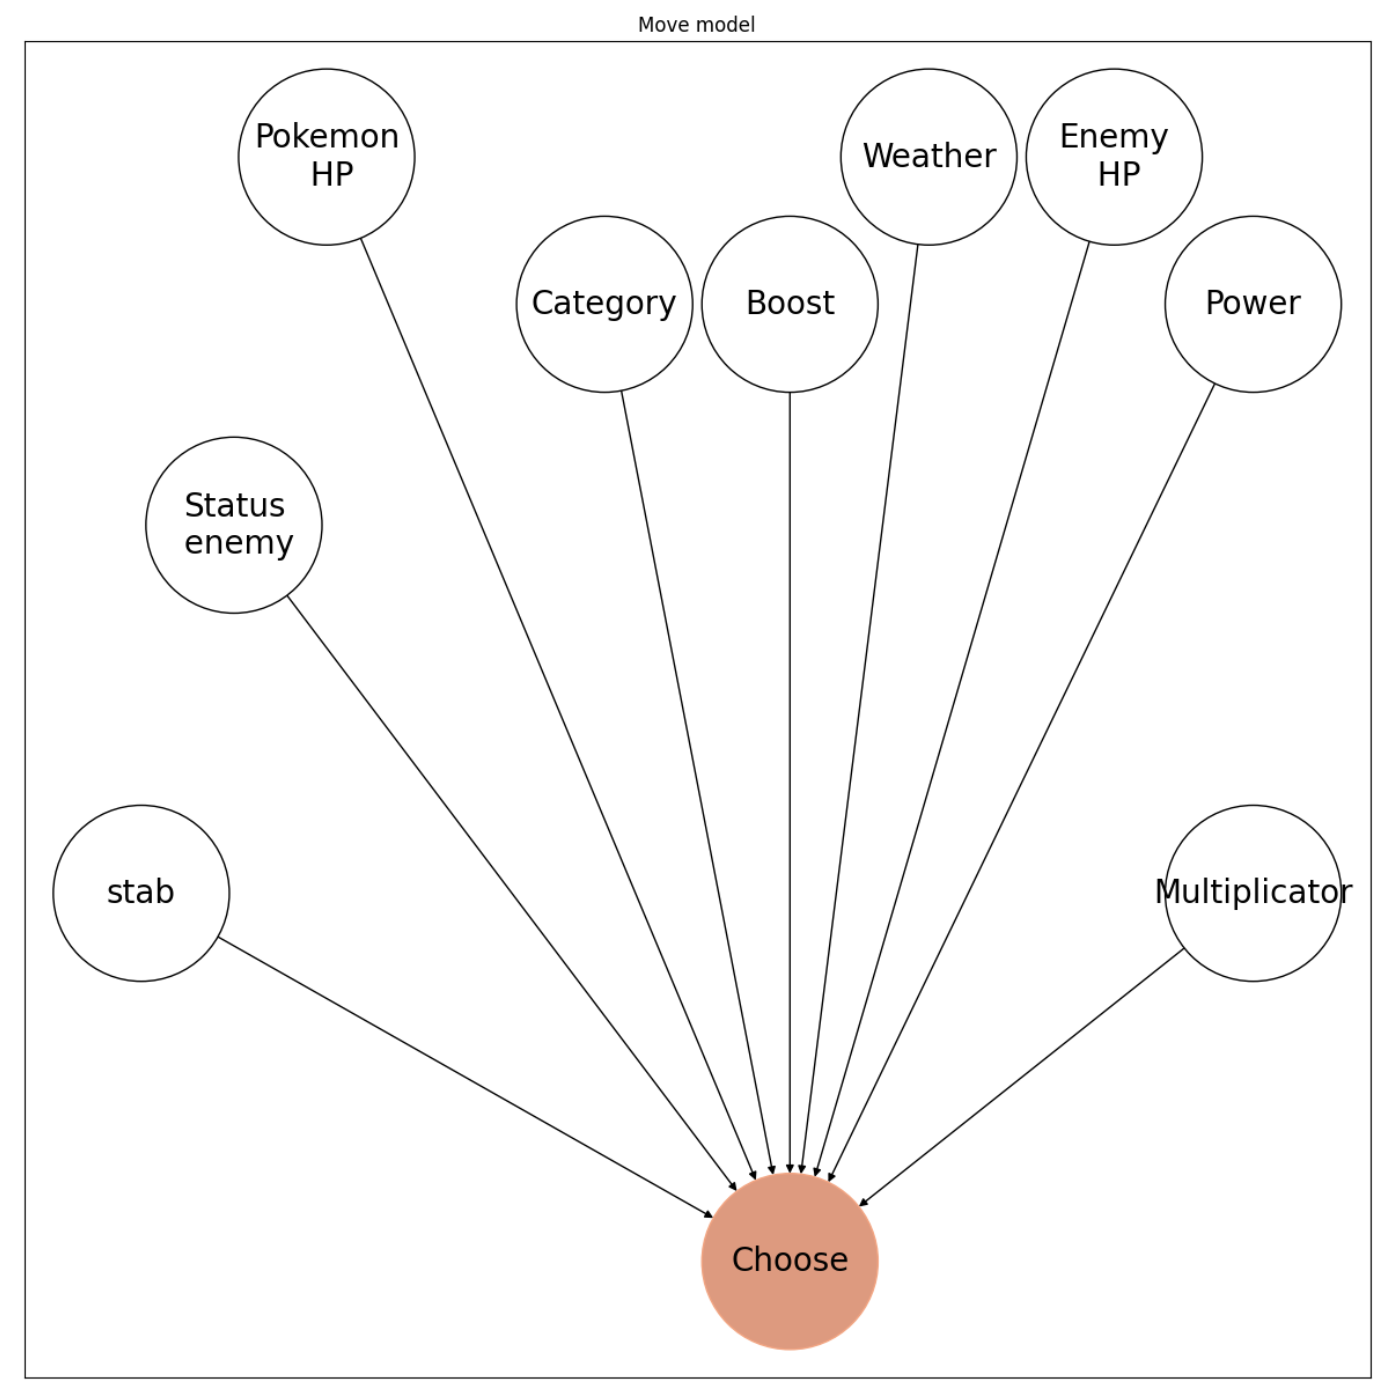
\includegraphics[width=.27\textwidth]{report/Move_bn_white.png}}
  \subfloat{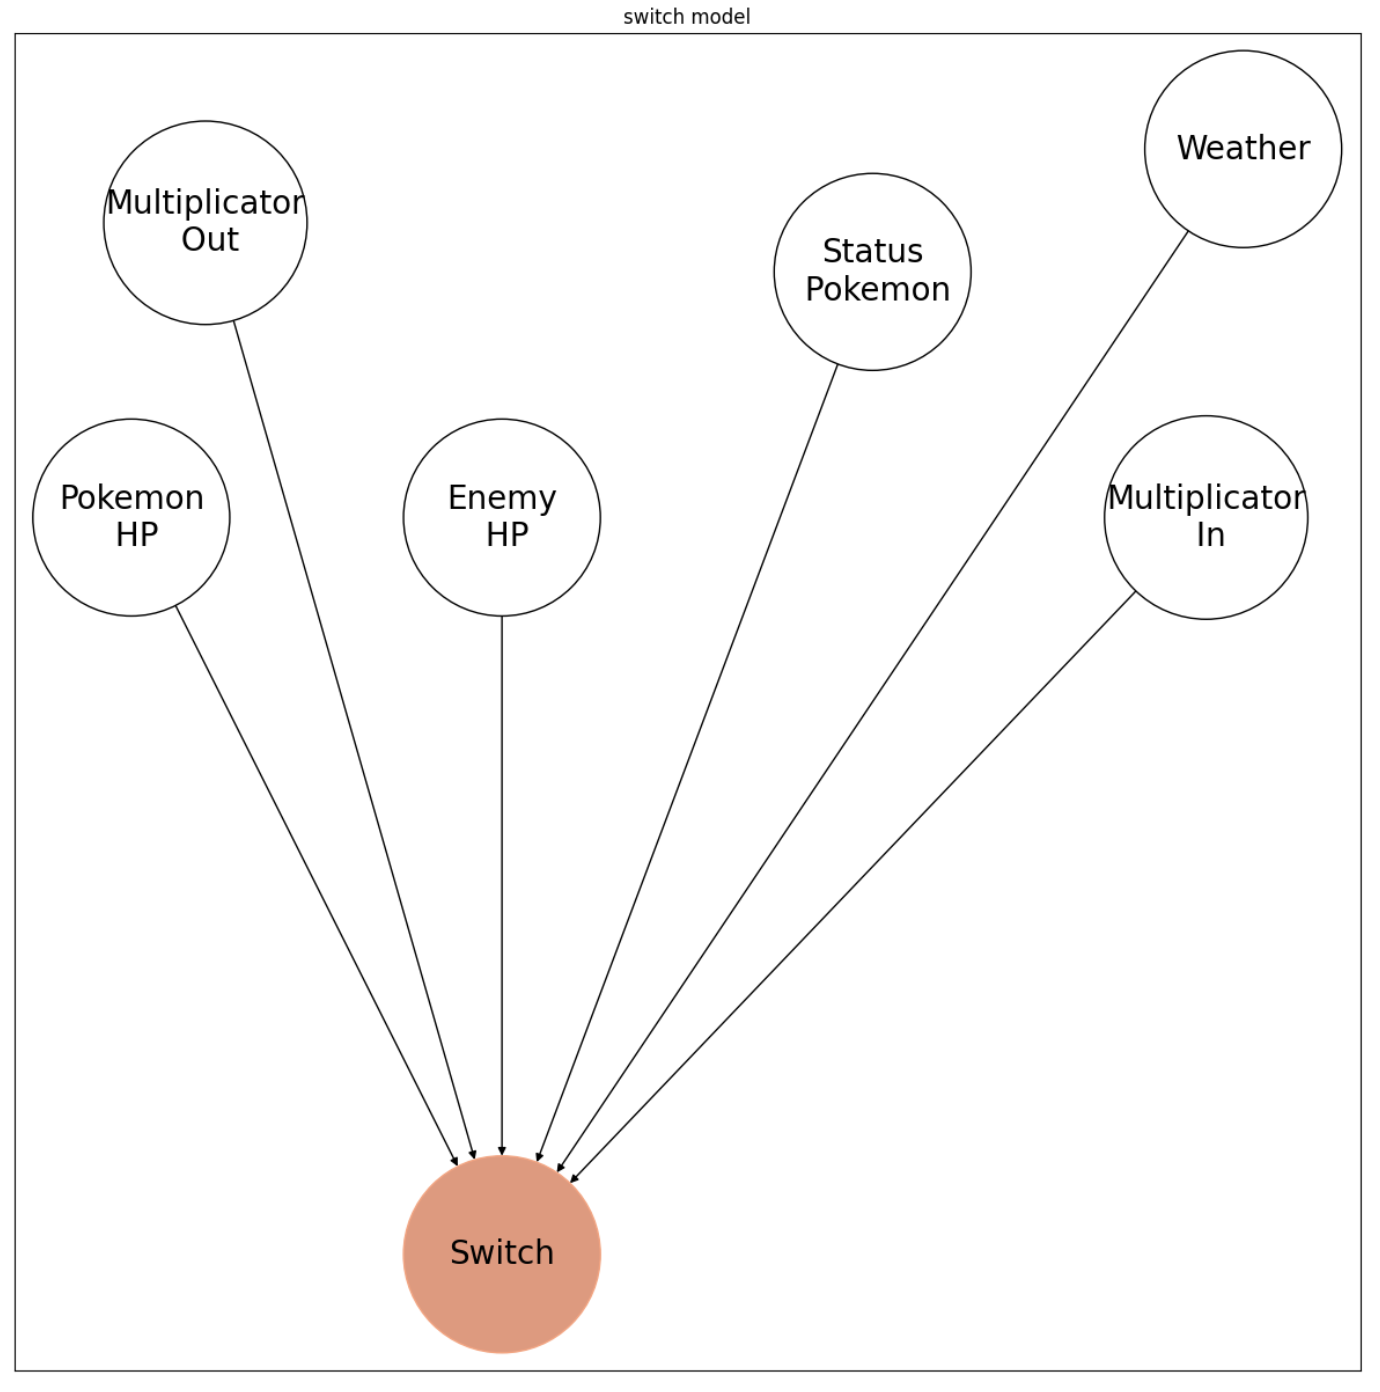
\includegraphics[width=.27\textwidth]{report/switch_bn_white.png}}
  
   \caption{The two Bayesian Network.}
  \label{fig:sub1}
\end{figure}

\begin{figure}[!ht]
    \centering
    \subfloat{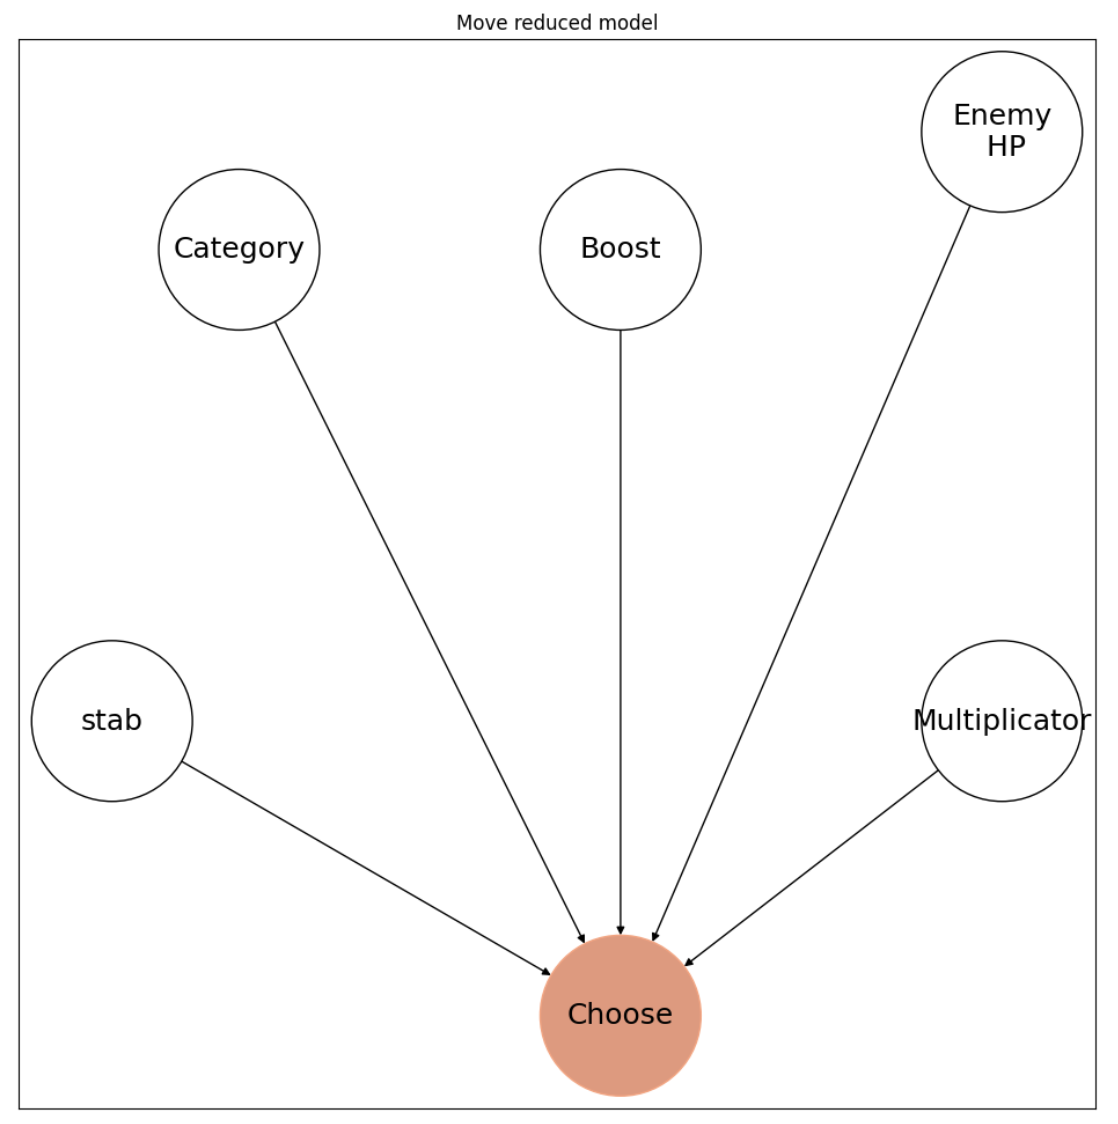
\includegraphics[width=.27\textwidth]{report/MoveREDU_bn_white.png}}
  \subfloat{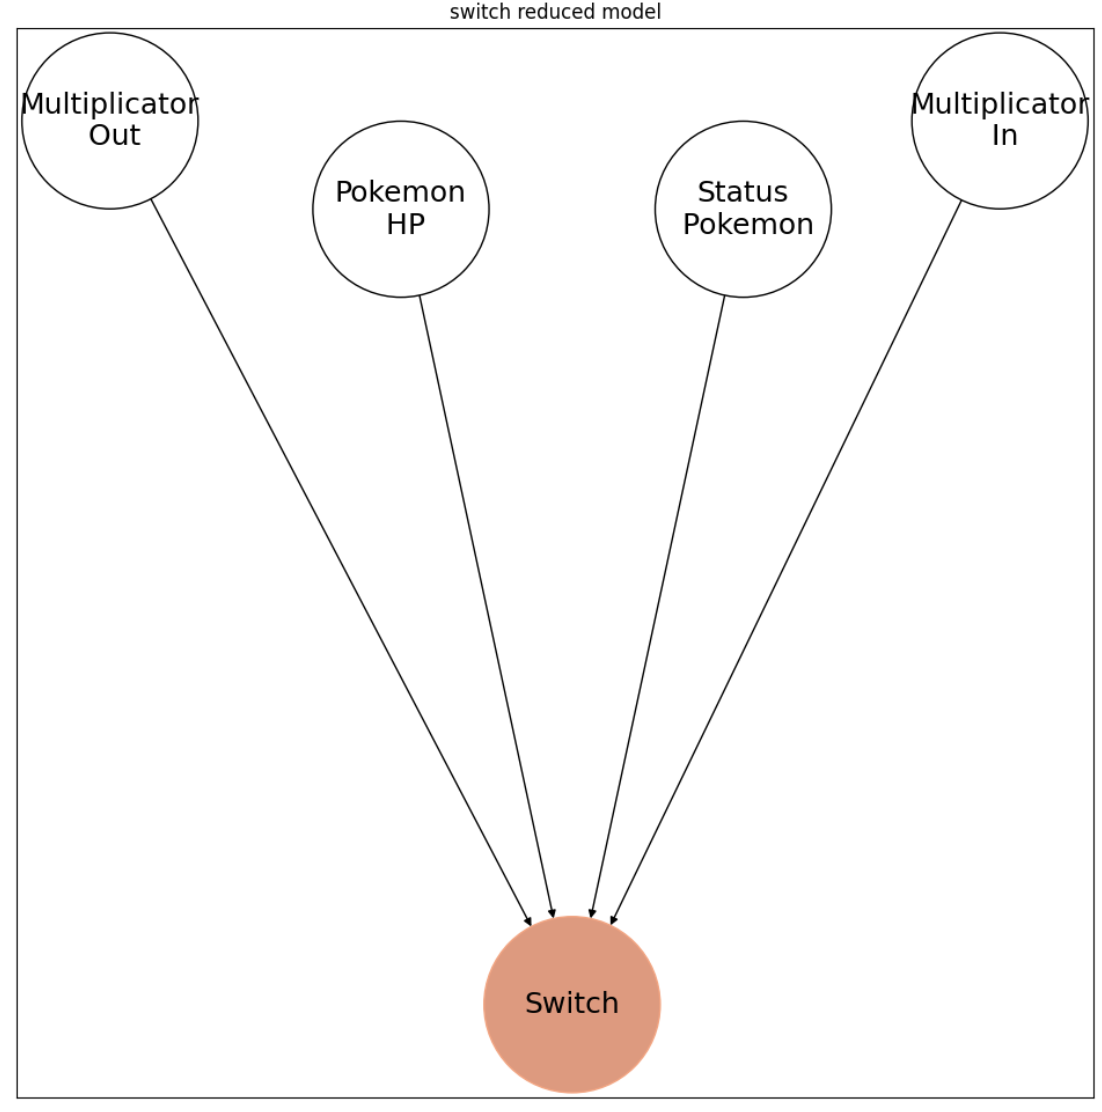
\includegraphics[width=.27\textwidth]{report/switchREDU_bn_white.png}}
  \caption{The two reduced Bayesian Networks.}
  \label{fig:sub1}
\end{figure}

\explanation{
Explain the following aspects of your model (if there is too much to say and not enough space, put in your notebook whatever does not fit here):
\begin{itemize}
    \item nodes: if not self-explanatory, explain each random variable's meaning/intuition and type/range
    \item conditional distributions (for example, the CPTs, some or all of them)
    \item the procedure you followed to build your model (structure and conditional distributions): from reference paper? by analyzing the domain? learned from data? just assigned probability distributions arbitrarily? followed a particular methodology for building the network? ...
\end{itemize}  
In general, only write whatever is relevant and necessary to understand the rest of the report. Do not explain concepts seen in class or explained in textbooks. Do not describe models taken from textbook/literature/tutorials/libraries, like (for example) the Asia network. Instead, if you are using a model as-is: just insert a reference or URL\footnote{\url{https://www.bnlearn.com/bnrepository/}.}
}

\section{Analysis}

\subsection{Experimental setup}
For every move and switch, we run a query on the corresponding BN to predict the "choose" or "switch" variable, given the evidence, which is the current state of the game, then the program will select the choice with the highest probability of being the best one.
The first comparison method is with a classical AI method for games, Iterative deepening, this was already implemented in the project from which we forked \cite{bot}.
To assess the results we have decided to create another version of the network, with a smaller number of variables and also some variables with a smaller number of values. We aim to compare these two versions to find out how much the size of the network affects their performances; to do this we let the models play against 100 people each in online battles and we compared the result to see which one had the most victory.
\explanation{
Briefly describe the probability queries or other experiments that you have carried out. Describe how you plan to evaluate the results (for example: are there results that you would expect?)
}

\subsection{Results}
In the table have been reported the results of the battles, as we can observe from the table, the best result has been obtained from the Iterative Deepening, followed by the "Reduced Bayesian Network", while the worst method has been proved to be the BN with the higher number of variables. This result was predictable since the limited, and not so diversified, amount of data we had could limit the BN favouring the iterative deepening, which do not need a training phase since it is a search strategy algorithm.
\begin{table}[h]
    \small
    \centering
    \begin{tabular}{lcrr}
        \hline \\[-1.8ex] 
        \hline \\[-1.8ex] 
        \textbf{} & \textbf{Match}  & \textbf{Win} & \textbf{Lost}\\
        \hline \\[-1.8ex] 
        \textbf{Bayesian Network}           &100   &21  &79\\
        \hline \\[-1.8ex] 
        \textbf{Reduced Bayesian Network}   &100  &31  &69\\
        \hline \\[-1.8ex] 
        \textbf{Iterative Deepening}        &100  &59  &41\\
        \hline \\[-1.8ex] 
        
    \end{tabular}
    \caption{Overview of the results of the battles} 
    \label{tab:libraries}
\end{table}

\explanation{
What did you observe? \\
%
All according to expectations? \\
%
Anything surprising or worthwhile mentioning?
}

\section{Conclusion}
After the Analysis of the result, it has been concluded that, in this case, the Bayesian Network with less variable is more accurate than the bigger one. This is probably because the bigger network has a large domain of possible state, this lead to every single state having a lower chance on happening, so the network can't distinguish well the different situation and tends to give equal probability for every move or possible switch. Because of this the bot tend to choose a random action and so not performing well. Instead the reduced one has less possible state, so the network know well most of the them, resulting in more decisive probability for most of the move. However, despite this increase in accuracy, the reduced network still perform worse than the iterative deepening, the cause of this, could probably resides in the structure of the Bayesian networks that can't describe well the domain.

\explanation{
Just one paragraph: what you have learned, anything interesting that came up, what are the limitations of your model/experiments/study/...
}

\section{Links to external resources}
The Dataset, the notebook containing the project and the implementation to let the bot play are available on \href{https://github.com/TechRufy/showdownBayesian.git}{GitHub}.
\explanation{
Optionally, insert here:
\begin{itemize}
    \item a link to your GitHub or any other public repo where one can find your code (only if you did not submit your code on Virtuale) 
    \item a link to your dataset (only if you have used a dataset, for example, for learning network parameters or structure)
\end{itemize}
Leave this section empty if you have all your resources in Virtuale. \textbf{Do not insert code/outputs in this report}.
}
\bigskip

\bibliographystyle{aaai}
\bibliography{faikrmod3.bib}


\attention{NOTICE: THIS REPORT'S LENGTH MUST NOT EXCEED \textbf{TWO PAGES} PLUS REFERENCES. THIS MAY MEAN THAT YOU WILL HAVE TO LEAVE OUT OF THE REPORT PART OF THE WORK YOU HAVE DONE OR OBSERVATIONS YOU HAVE. THIS IS NORMAL: THE REPORT SHOULD EMPHASIZE WHAT IS MOST SIGNIFICANT, NOTEWORTHY, AND REFER TO THE NOTEBOOK FOR ANYTHING ELSE. FOR ANY OTHER ASPECT OF YOUR WORK THAT YOU WOULD LIKE TO EMPHASIZE BUT CANNOT EXPLAIN HERE FOR LACK OF SPACE, FEEL FREE TO ADD COMMENTS IN THE NOTEBOOK.}


\end{document}